\documentclass{myformat}
\addbibresource{mylib.bib}


\makeglossaries

\setabbreviationstyle[acronym]{long-postshort-user}
\glssetcategoryattribute{acronym}{nohyperfirst}{true}
\setabbreviationstyle{short-nolong}

\newglossaryentry{asyncio}{name=thing,description={A Python library for asynchronous code using coroutines, event loops, and tasks.}}
% --------------------
% ----- Acronyms -----
% --------------------

\newacronym{nvs}{NVS}{Novel View Synthesis}
\newacronym{mlp}{MLP}{Multi-Layer Perceptron}
\newacronym{nerf}{NeRF}{Neural Radiance Field}
\newacronym{rt}{RT}{Ray Tracing}
\newacronym{bvh}{BVH}{Bounding Volume Hierarchy}

% \glsaddall
% \glsunset{cpu}
% \glsunset{gpu}
% \glsunset{lla}
% --------------------
% ----- Shortcuts ----
% --------------------


\newcommand{\nvidia}{NVIDIA\xspace}

\newcommand{\jetson}{\gls{jetson}\xspace}
\newcommand{\sr}{Sensor Rig\xspace}
\newcommand{\jx}{Xavier\xspace}
\newcommand{\jo}{Orin\xspace}
\newcommand{\gs}{Gstreamer\xspace}
\newcommand{\cam}{Triton Polarizin Camera\xspace}
\newcommand{\cams}{Triton Polarizin Cameras\xspace}
\newcommand{\lucid}{Lucid Vision\xspace}
\newcommand{\preproject}{Pre-Project\xspace}
\newcommand{\master}{Master's\xspace}
\newcommand{\py}{Python\xspace}
\newcommand{\cpu}{\gls{gpu}\xspace}
\newcommand{\gpu}{\gls{cpu}\xspace}
\newcommand{\gui}{GUI\xspace}
\newcommand{\guif}{\gls{gui} framework\xspace}
\newcommand{\srgui}{\sr \gls{gui}\xspace}


\begin{document}


\title{Gaussian Splatting \\ The Future of 3D World Representation?}

\author{Emil Martens}
\markboth{Journal of \LaTeX\ Class Files,~Vol.~14, No.~8, August~2015}{}
\maketitle

\begin{abstract}
    The introduction of Gaussian Splatting has disrupted the field \gls{nvs}. This technology has gained rapid adoption and further development in academia, and it has also been successfully leveraged in the industry, showcasing its immense potential \cite{LumaAIVideo}.

    This report aims to provide an accessible overview of the paper that introduced Gaussian Splatting and discuss its implications.
    Additionally, we will explore hypothetical future improvements to the core technology by harnessing the power of hardware-accelerated ray tracing and polarization cameras.


\end{abstract}

\section{Introduction}
\gls{nvs} is a computer vision problem where the goal is to represent a scene in a way such that given a new \text{view}, an accurate image can be generated.
Here we define a \textit{view} as the position and orientation of a camera in the scene together with the camera's intrinsic parameters.

Current state-of-the-art methods vary in how they represent the scene and generate images
but share the same general problem formulation;
Given a set of training images $\bm{I}_i$,
taken from different views $\bm{V}_i$,
the goal is to find a representation of the scene $\bm{S}$,
together with a image generating function $\bm{\hat{I}}_i = g(\bm{S}, \bm{V}_i)$,
such that some cost function $\mathcal{L}(\bm{I}_i, \bm{\hat{I}}_i)$,
is minimized over all training images.

To evaluate the performance of a method, a collection of test images $\bm{I}_j$ together with their corresponding views $\bm{V}_j$ is used to evaluate the method's ability to generalize to unseen data.
Beyond a method's ability to accurately generate images from novel views, other important metrics should be considered.
This includes the time it takes to generate an image, the memory required to store the scene representation, the time it takes to train the model, the amount of training data required and the amount of memory required during training.



\section{Previous Work}
\gls{nvs} is a well-studied problem in computer vision, and many different approaches have been proposed.
Older methods achieved decent image interpolation by estimating the depth of the scene to correctly warp and blend adjacent images \cite{zitnickHighqualityVideoView2004}.
The

% With the development of \gls{sfm} methods
the introduction of \gls{nerf} methods had a big  \cite{mildenhallNeRFRepresentingScenes2020a}.




Older methods have achieved good image interpolation by estimating the depth of the scene and use warping and blending to generate new images \cite{zitnickHighqualityVideoView2004}.

Recent \gls{nerf} methods build a continuous representation of the scene, usually by optimizing a neural network to predict the radiance at any point in space \cite{mildenhallNeRFRepresentingScenes2020a}.
Ray marching is used to sample points from the scene to render the scene from a given viewpoint.
A problem with this approach is that a lot of resources are wasted on rendering transparent or occluded parts of the scene, as the whole volume is sampled.
Different new representations have been proposed to circumvent this problem, including using a sparse voxel grid \cite{yuPlenoxelsRadianceFields2021a}, a hash table \cite{mullerInstantNeuralGraphics2022} and points \cite{xuPointNeRFPointbasedNeural2023}.
However, none of these methods appear to perform as well as the method proposed in the Gaussian Splatter paper, where they represent the scene using a set of Gaussian splats \cite{kerbl3DGaussianSplatting2023}.





\section{Paper Summary}

\begin{figure*}
    \centering
    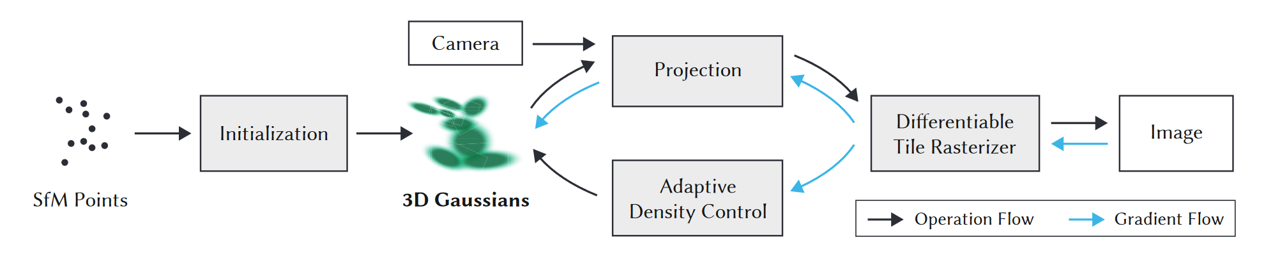
\includegraphics[width=\textwidth]{images/pipeline.png}
    \caption{The Gaussian splatting pipeline presented in the paper \cite[Fig. 2]{kerbl3DGaussianSplatting2023}.}
\end{figure*}


\subsection{Representation}
The core idea of the paper is to represent the scene as a set of Gaussians.
Each Gaussian is defined by its position $\bm{p}$, its covariance matrix $\bm{\Sigma}$, its color $\bm{c}$ and its opacity $\alpha$.

As the covariance has to be symmetric and positive definite, it is defined as
\begin{align}
    \bm{\Sigma} = \bm{R} \bm{S} \bm{S}^T \bm{R}^T,
\end{align}
where $\bm{R}$ is a rotation matrix stored as a quaternion $\bm{q}$ and $\bm{S}$ is a diagonal matrix containing the standard deviation of the Gaussian along each axis stored as a vector $\bm{s}$
To ensure that the covariance is positive definite, the diagonal elements of $\bm{S}$ are passed through a sigmoid function.
The quaternion $\bm{q}$ is normalized to ensure a proper rotation matrix.

% Similarly to other \cite{yuPlenoxelsRadianceFields2021a}\cite{mullerInstantNeuralGraphics2022}


\subsubsection{Spherical Harmonics}
\begin{figure}
    \centering
    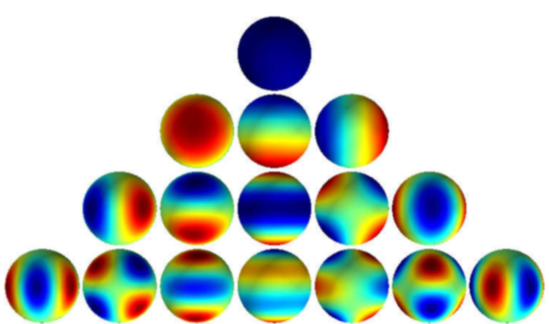
\includegraphics[width=\linewidth]{images/spherical_harmonics.png}
    \caption{Visualization of the spherical harmonics used to represent the view-dependent color of each Gaussian \cite[Fig. 3]{kerbl3DGaussianSplatting2023}.}
\end{figure}

\subsubsection{Camera Projection}

\subsection{Rasterization Pipeline}
\begin{figure}
    \centering
    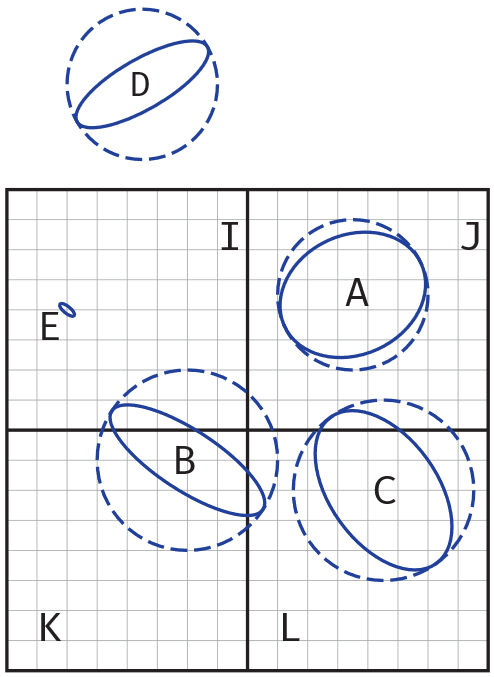
\includegraphics[width=0.6\linewidth]{images/rendering.png}
    \caption{Visualization of how Gaussian splats are rendered using multiple independent blocks.}
\end{figure}
\label{sec:rasterization}

\subsection{Densification}
\begin{figure}
    \centering
    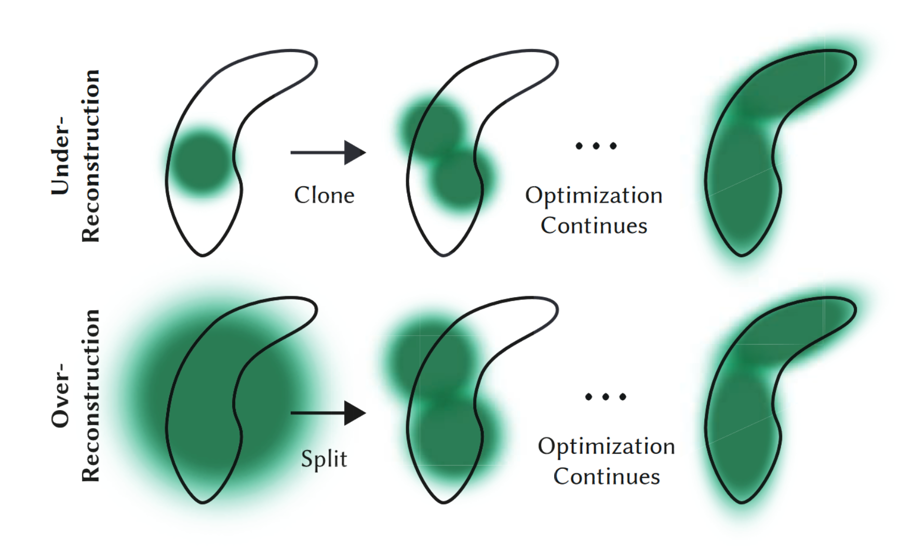
\includegraphics[width=\linewidth]{images/densification.png}
    \caption{The adaptive Gaussian densification scheme presented in the paper \cite[Fig. 4]{kerbl3DGaussianSplatting2023}.}
\end{figure}

\section{Critique and Potential Improvements}
In this section, we will discuss certain elements of the paper that we believe could be improved.

\subsection{Spherical Harmonics}
In the current implementation, they use spherical harmonics to handle view-dependent color from reflections.
They present this approach as "following standard practice" referencing the Plenoxels and Instant Neural Graphics papers \cite{yuPlenoxelsRadianceFields2021a}\cite{mullerInstantNeuralGraphics2022}.
As the paper uses a fundamentally different representation of the scene, I believe following the same approach for view-dependent color might not be the best choice.

The other methods both use some voxel-based representation of the scene,
where the sampling of each point is independent of the view direction,
making it necessary for each point to contain view-dependent color \cite{yuPlenoxelsRadianceFields2021a}\cite{mullerInstantNeuralGraphics2022}.
In the Gaussian splatting method, a discrete set of Gaussians is used to represent the scene, which could be leveraged to avoid the need for view dependence, by having overlapping Gaussians with view-dependent opacity.
This could be used to have Gaussians that are only visible from a narrow range of view directions, placed in front of the scene geometry to simulate reflections.

The paper shows that even without spherical harmonics, the scene converges to a good result \cite[Table 3]{kerbl3DGaussianSplatting2023}.
We propose to remove the spherical harmonic coefficients from the representation of each Gaussian, reducing the parameter number from 60 to 15 and adding a second phase to the rendering pipeline to handle reflections.
In this phase, we keep the converged scene constant and add a set of Gaussians with a view-dependent opacity to simulate reflections.

A potential problem with this approach is the popping effect discussed in Section \ref{sec:popping}, which makes it difficult to optimize Gaussians laying on the surface of the scene geometry.

\subsection{Use CUDA Streams to increase parallelism}
The code provided by the authors showcases a deep understanding of CUDA and GPU architecture,
notably in the way they ensure memory coalescing, avoid bank conflicts and leverage shared memory in the rasterization pipeline.
This makes it surprising that they do not use CUDA streams to increase parallelism.
When running the code on a workstation with an i9-13900KF CPU and an RTX 4090 GPU the GPU utilization was only around 30\% as the training process was severely bottlenecked by the single-threaded CPU code.
In the paper, they acknowledge that the majority (~80\%) of the training time is spent in Python code, and argue it is a necessary tradeoff to allow for easy adoption by other researchers \cite[Sec. 8]{kerbl3DGaussianSplatting2023}.
While the adaptability of the code is appreciated, it does not explain why they did not use CUDA Streams to increase parallelism, as Streams have deep support in PyTorch and can easily be disabled even if support is implemented \cite{pytorchcontributorsCUDASemanticsPyTorch2023}.

\subsection{Regularization}
The paper acknowledges that the optimized Gaussians tend to be very non-isotropic, i.e. very stretched out, as  Regularization is not performed \cite[Sec. 7.4]{kerbl3DGaussianSplatting2023}.
This is illustrated in Figure \ref{fig:very_isotropic}.
One way to solve this would be to add a cost based on the index of dispersion of the scale parameters $\bm{s}$ of each Gaussian, that is the ratio of the variance to the mean, which would have a value of 0 for spherical Gaussians.

\begin{figure}
    \centering
    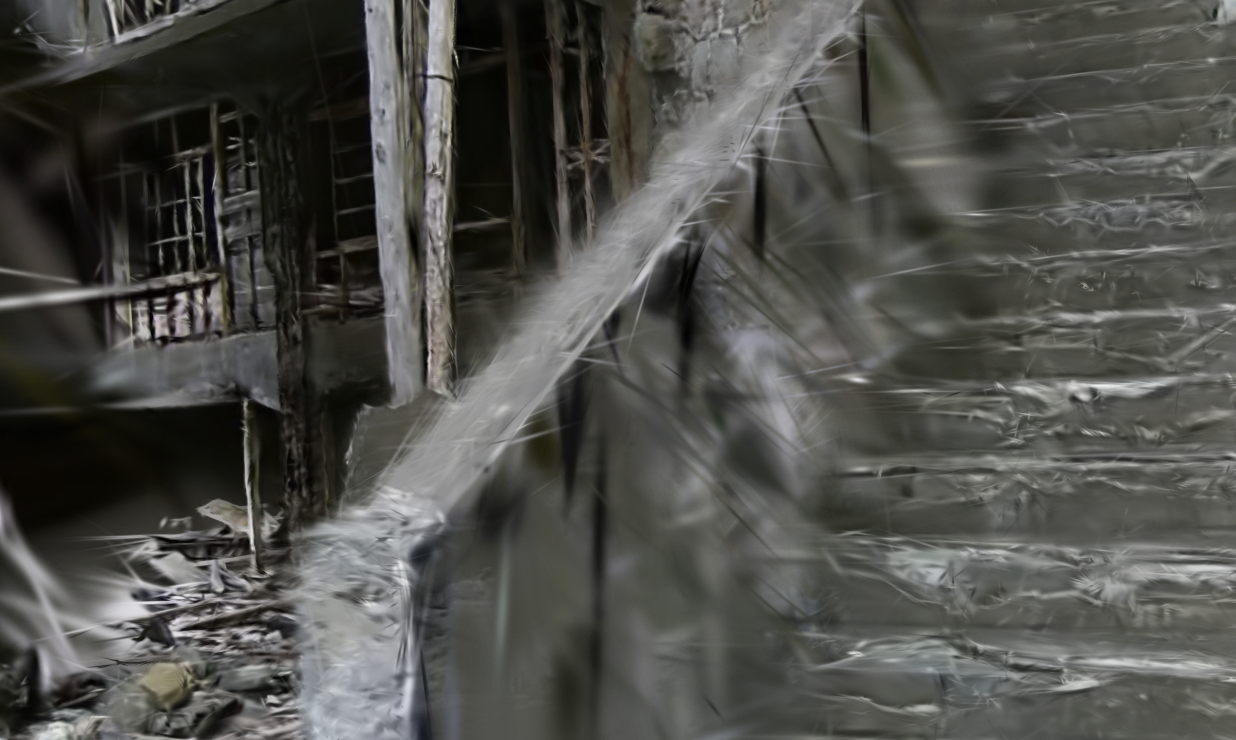
\includegraphics[width=\linewidth]{images/very_isotropic.png}
    \caption{Going outside the captured view angles illustrate how non-isotropic the Gaussians are \cite{@nekoHashimaIslandCreated2023}}
    \label{fig:very_isotropic}
\end{figure}

\subsection{Gaussian}
Why they chose to use a Gaussian to represent the scene is not explained in the paper.
As there is no connection to statistics or probability theory, it seems like an arbitrary choice.


\section{Potential benefits of ray tracing}
Going away from the current rasterization-based rendering pipeline and instead using ray tracing to render the scene has many potential benefits.

\subsection{Ray Tracing}
Ray tracing is a rendering technique that simulates the path of light rays through a scene.
While rasterization is limited to rendering a scene from one viewpoint at a time, by projecting the scene onto a two-dimensional plane, ray tracing is not limited in this way \cite{caulfieldWhatPathTracing2022}
As such, ray tracing can be used to perform path tracing, which is a physically based rendering technique that simulates the path of light rays through a scene \cite{caulfieldWhatPathTracing2022}.

As ray tracing has become a key component of rendering in the gaming industry, specialized hardware has been developed to accelerate the process.
Modern NVIDIA GPUs have dedicated \gls{rt} cores that can be used to accelerate ray tracing through the NVIDIA OptiX\textsuperscript{TM} API \cite{nvidiaNVIDIAOptiXProgramming2023}.

A ray tracing pipeline consists of three main steps creating an acceleration structure,


\subsection{Better Representation}
In the current representation of each Gaussian, several extra steps are required to guarantee correctness.

\subsection{Reflections}
Reflections in the scene pose a significant challenge in the field of \gls{nvs}, as it requires the ability to capture view-dependent color.
As discussed earlier, the use of spherical harmonics solves this to some degree, but it comes at a significant memory cost.
When using ray tracing, it might be possible to circumvent the need for view-dependent color by using ray-traced reflections.

Without the use of ray tracing cores, this is impossible, as the whole rendering pipeline for the Gaussian splats, discussed in Section \ref{sec:rasterization}, would have to be performed for each reflected ray as they would not share the same origin.
This would make the rendering process several million times slower.

However, with the use of ray tracing cores, rendering a reflected ray is no different than rendering a regular ray \footnote{It might be slightly worse due to data locality, but this should be handled by the hardware.}.


Using polarization cameras might prove very useful in this regard, as reflected light has a distinct polarization signature \cite{lingUniversityPhysicsVolume2016}.




The simple approach would be to remove reflected light from the scene and partially circumvent the need for view-dependent color.
This approach only targets the input data and should thus be easy to evaluate using the implementation from the paper.
The results from this approach will however look different than what a regular camera would capture, as the reflected light is partially removed.

Another, arguably more interesting, approach would be to use the polarization information to estimate the surface normal of each triangle and calculate ray-traced reflections.
As the polarization cameras can capture the angle of polarization for each pixel, using multiple views it should be possible to estimate the three-dimensional surface normals with some degree of accuracy.
This approach has been presented by one manufacturer of polarization cameras as shown in Figure \ref{fig:polarization} \cite{lucidvisionlabs3DDepthSurface2021}.





\begin{figure}
    \centering
    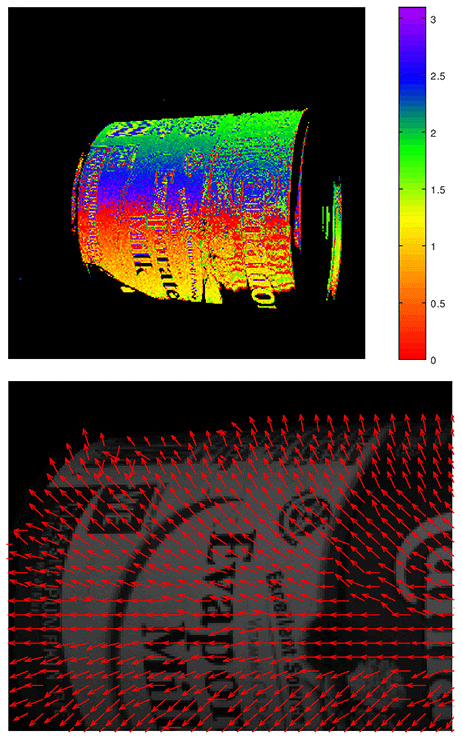
\includegraphics[width=\linewidth]{images/polarization_normals.png}
    \caption{Angle of orientation and estimated surface normals from polarized light \cite{lucidvisionlabs3DDepthSurface2021}}.
    \label{fig:polarization}
\end{figure}






\subsection{Code closer to Problem formulation}
There is a significant difference between how the problem is formulated in the paper and how
\section{Conclusion}
Gaussian splatting is a promising new method for \gls{nvs} that has shown impressive results.
The core idea of the method is to go back from the continuous representation of the scene used in \gls{nerf} related methods and instead represent the scene as a discrete set of Gaussians.
While the paper, its public implementation and the shown result are impressive, we did find some areas where we believe the method could be improved.

Taking inspiration from the paper, we proposed a new path for \gls{nvs} where we leverage the power of modern hardware-accelerated ray tracing.
We believe this could be a promising path for \gls{nvs} that will synergize well with the recent development of polarization cameras.

% \glsaddall


% \printglossary[type=\acronymtype]
\printglossaries
\printbibliography

\end{document}